\begin{figure}[t]
\centering
  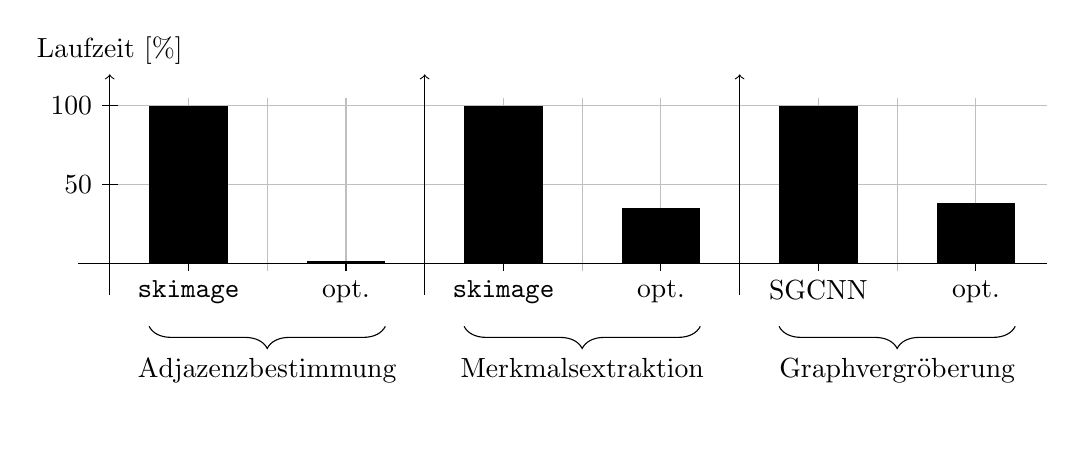
\begin{tikzpicture}[]
  \fill[white] (0, -2) rectangle (1, -1) node {};  % Abstand nach unten

  \draw[color=lightgray] (-0.1, -0.1) grid (11.9, 2.1);

  \draw[] (-0.4, 0) -- (11.9, 0);
  \draw[->] (0, -0.4) -- (0, 2.4) node[above] {Laufzeit [\%]};
  \draw[->] (4, -0.4) -- (4, 2.4);
  \draw[->] (8, -0.4) -- (8, 2.4);

  \draw (0.1, 1) -- (-0.1, 1) node[left] {$50$};
  \draw (0.1, 2) -- (-0.1, 2) node[left] {$100$};

  \draw[line width=1cm] (1, 0) -- (1, 2);
  \draw[line width=1cm] (3, 0) -- (3, 0.030153);
  \draw (1, 0) -- (1, -0.1) node[below] {\texttt{skimage}};
  \draw (3, 0) -- (3, -0.1) node[below] {opt.};
  \draw [decoration={brace,mirror,amplitude=8pt},decorate] (0.5,-0.8) -- node[below=8pt] {Adjazenzbestimmung} (3.5,-0.8);

  \draw[line width=1cm] (5, 0) -- (5, 2);
  \draw[line width=1cm] (7, 0) -- (7, 0.704036);
  \draw (5, 0) -- (5, -0.1)  node[below] {\texttt{skimage}};
  \draw (7, 0) -- (7,  -0.1) node[below] {opt.};
  \draw [decoration={brace,mirror,amplitude=8pt},decorate] (4.5,-0.8) -- node[below=8pt] {Merkmalsextraktion} (7.5,-0.8);

  \draw[line width=1cm] (9, 0)   -- (9, 2);
  \draw[line width=1cm] (11,  0) -- (11,  0.769867);
  \draw (9, 0)  -- (9, -0.1)  node[below] {\acs{SGCNN}};
  \draw (11, 0) -- (11, -0.1) node[below] {opt.};
  \draw [decoration={brace,mirror,amplitude=8pt},decorate] (8.5,-0.8) -- node[below=8pt] {Graphvergröberung} (11.5,-0.8);

\end{tikzpicture}

\begin{tabular}{lrrr}
  \toprule
  Vorverarbeitungsschritt & vorhanden [ms] & optimiert [ms] & Gewinn [\%]\\
  \midrule
  Adjazenzbestimmung & 866 & 13 & 6615\\
  Merkmalsextraktion & 144 & 50 & 288\\
  Graphvergröberung (4 Ebenen) & 87 & 33 & 264\\
  \bottomrule
\end{tabular}

\caption[Laufzeitvergleich \bzgl{} anderer Implementierungen]{Vergleich der Laufzeiten verschiedener Vorverarbeitungsschritte \bzgl{} des Lernens auf Graphen zwischen bereits vorhandenen, quelloffenen Implementierungen (links) und ihren jeweiligen entwickelten optimierten Versionen (rechts) am Beispiel eines Bildes aus \gls{Pascal}: (1) Adjazenzbestimmung einer Segmentierungsmaske, (2) Merkmalsextraktion und (3) Graphvergröberung inklusive der entsprechenden Anordung der Knoten zu binären Bäumen.
  In allen Bereichen konnten deutliche Laufzeitgewinne erreicht werden.}
\label{fig:laufzeit_vergleich}
\end{figure}
